\documentclass[a4paper]{article}
\author{Zhenhao Li}
\title{\textbf{CO-496 Coursework\ \#4}}

\usepackage{amsmath,bm}
\usepackage{graphicx}
\usepackage{grffile}
\usepackage{geometry}

\geometry{a4paper,scale=0.8}


% --------取消自动换行--------
\tolerance=1
\emergencystretch=\maxdimen
\hyphenpenalty=10000
\hbadness=10000
% --------------------------

\begin{document}
\maketitle

\section*{Part I}

\begin{figure}[htb]
   \begin{minipage}{0.33\textwidth}
     \centering
     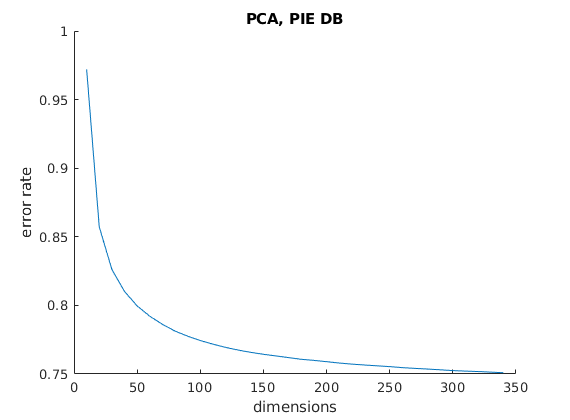
\includegraphics[width=1\linewidth]{../pic/PCA.png}
     \caption{PCA}\label{Fig:PCA}
   \end{minipage}\hfill
   \begin{minipage}{0.33\textwidth}
     \centering
     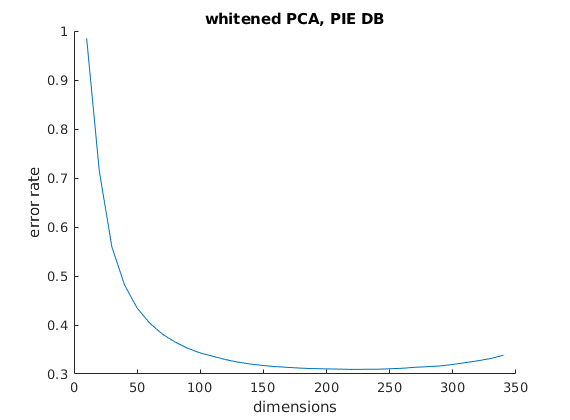
\includegraphics[width=1\linewidth]{../pic/wPCA.png}
     \caption{wPCA}\label{Fig:wPCA}
   \end{minipage}
   \begin{minipage}{0.33\textwidth}
     \centering
     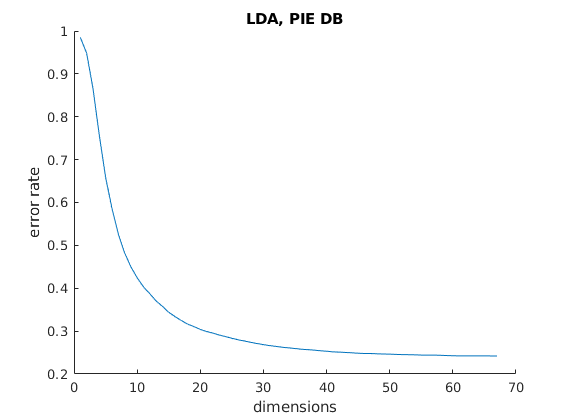
\includegraphics[width=1\linewidth]{../pic/LDA.png}
     \caption{LDA}\label{Fig:LDA}
   \end{minipage}
\end{figure}

\begin{itemize}
    \item{From the three plots, LDA achieves the best performace and the error rate reduces to below 0.3 .}
    \item{The wPCA method performs better than the PCA method because it normalizes the data, setting the covariance matrix of the data equal to identity matrix. However, when the number of dimensions is over 250, the error rates of wPCA starts to raise back. This is possibly because the features of trivial eigenvalues are taken into consideration and they plays few help in representing the data. Since wPCA normalizes features on every dimension, these features are of same importance as those really "important" features.}
    \item{The input labels are important in reducing the error rate of LDA. PCA or wPCA are unsupervised methods while LDA is a supervised method. Therefore, with the same dataset, LDA can utilize more infomation than the former two, which results in lower error rates. }
\end{itemize}

\section*{Part II}
\textbf{1.} Formulate the Lagrangian of the above optimisation problem and derive its dual.
Attach your answers in the report. Show the steps that you followed, do not only
report the final results.\\
\\
The Lagrangian is
\begin{equation}
    L(R,\bm a,\xi_i,t_i,r_i) = R^2 + C\sum_{i=1}^{n}\xi_i + \sum_{i=1}^{n}t_i\big((\bm{x_i}-\bm{a})^T(\bm{x_i}-\bm{a})-R^2-\xi_i\big) - \sum_{i=1}^{n}r_i\xi_i
\end{equation}
with Lagrangian multiplier $t_i \geq 0, r_i \geq 0$. Computing the derivatives
\begin{equation}
    \begin{aligned}
        &\frac{\partial L}{\partial R} = 2R - 2R \sum_{i=1}^{n}t_i = 0 \\
        &\frac{\partial L}{\partial \bm a} = \sum_{i=1}^{n}t_i(2\bm a - 2\bm{x_i})=0\\
        &\frac{\partial L}{\partial \xi_i} = C-t_i-r_i = 0\\
    \end{aligned}
\end{equation}
Substituting (2) back into (1) we get the dual optimisation problem
\begin{equation}
    \begin{aligned}
        &\max_{\bm{t}}L(\bm t) = \bm k^T \bm t - \bm{t}^T\bm{X}^T\bm{Xt}\\
        & subject\ to\ \bm t^T\bm 1 = 1, 0 \leq t_i \leq C\\
        & where\ \bm k = [||x_1||_2^2, ... ,||x_n||_2^2]^T
    \end{aligned}
\end{equation}
\\
\\
\textbf{2.} Perform the above when using arbitrary positive definite kernels (i.e., $k(\bm x_i, \bm x_j) =
\phi(\bm x_i)^T\phi(\bm x_j)) $, i.e. find the dual of the following optimisation problem
\[
\begin{aligned}
    &\min_{R,\bm a,\xi_i} R^2 + C\sum^n_{i=1}\xi_i \\
    & subject\ to\ (\phi(\bm x_i) - \bm a)^T (\phi(\bm x_i) - \bm a) \leq R^2 + \xi_i, \forall \xi_i \geq 0
\end{aligned}
\]
Attach your answers in the report. Show the steps that you followed, do not only
report the final results.\\
\\
The Lagrangian is
\begin{equation}
    L(R,\bm a,\xi_i,t_i,r_i) = R^2 + C\sum_{i=1}^{n}\xi_i + \sum_{i=1}^{n}t_i\big((\phi(\bm{x}_i)-\bm{a})^T(\phi(\bm{x}_i)-\bm{a})-R^2-\xi_i\big) - \sum_{i=1}^{n}r_i\xi_i
\end{equation}
with Lagrangian multiplier $t_i \geq 0, r_i \geq 0$. Computing the derivatives
\begin{equation}
    \begin{aligned}
        &\frac{\partial L}{\partial R} = 2R - 2R \sum_{i=1}^{n}t_i = 0 \\
        &\frac{\partial L}{\partial \bm a} = \sum_{i=1}^{n}t_i(2\bm a - 2\phi(\bm{x}_i))=0\\
        &\frac{\partial L}{\partial \xi_i} = C-t_i-r_i = 0\\
    \end{aligned}
\end{equation}
Substituting (5) back into (4) we get the dual optimisation problem
\begin{equation}
    \begin{aligned}
        &\max_{\bm{t}}L(\bm t) = \bm k^T \bm t - \bm{t}^T\bm{\Phi}^T\bm{\Phi t}\\
        & subject\ to\ \bm t^T\bm 1 = 1, 0 \leq t_i \leq C \\
        & where\ \bm k = [k(\bm x_1, \bm x_1), ... ,k(\bm x_n, \bm x_n)]^T
    \end{aligned}
\end{equation}
\\
\\
\textbf{3.}\\
The centre and radius for the two classes are
\[
\begin{aligned}
    &\bm a_{red} = (0.0037, -0.0343) \\
    &R_{red} = 0.9866 \\
    &\bm a_{blue} = (-0.0036, 0.0015) \\
    &R_{blue} = 1.9835
\end{aligned}
\]

\begin{figure}[htb]
     \centering
     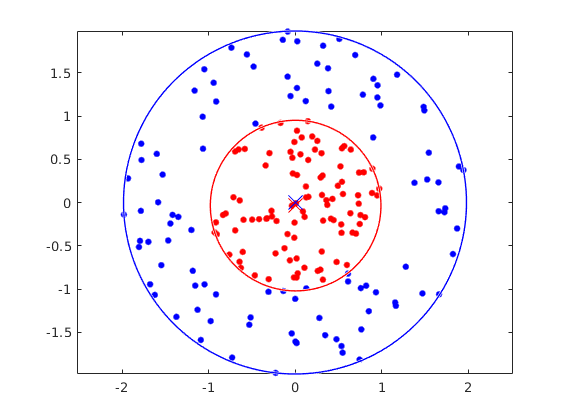
\includegraphics[width=1\linewidth]{../pic/SVM.png}
     \caption{SVM}\label{Fig:SVM}
\end{figure}
\end{document}
